\documentclass[../../main.tex]{subfiles}

\begin{document}

\section{Linear Transformations}

When we discussed about matrices, we saw that they kind of ``change''
the vector space. When I first learned about matrices in an academy
as a middle school student, all I had in mind was ``this is an
interesting way of organizing items!'' I knew what vectors and
matrices were, but I didn't really know them. That changed until
I learned about linear transformations. Of course, I wouldn't expect
my middle school self to learn all these and truly understand what
matrices represent in a vector space, but this moment, or section
really changed my understanding. Like all the other sections, this
is an interesting one, and let's get started!

\subsection{Brief Review of Functions}

Before we get into linear transformations, let's review about
functions. I think this would be a good refresher on the terms.

\begin{definition}{}{}
A \textbf{function} is a special \textbf{relation} where each input
from its domain has exactly one corresponding output.
\end{definition}

For instance, a function $f: X \to Y$ is a special relation whose
domain is $X$ and whose corresponding outputs lie in $Y$. As you
probably know, there are special terms for $X$ and $Y$.

\begin{definition}{}{}
The set of all inputs of a function is called \textbf{domain} of the
function. The set of all corresponding outputs is known as
\textbf{image}, or range, of the function denoted as $\Im(f)$.
\end{definition}

You might be familiar with the term \textbf{range}, but \textbf{image}
and \textbf{range} refer to the same thing, and \textbf{image} is
more commonly used in linear algebra and other courses. Now let's
review about bijection, injection, and surjection.

\begin{definition}{}{}
A function is \textbf{injective}, or one-to-one, if each element in
the domain maps to a unique element in the image. A function is
\textbf{surjective}, or onto, if the image and codomain are identical.
A \textbf{bijective} functions are functions that are both injective
and surjective.
\end{definition}

For more visual representation, below is a diagram that manifests
the definition above.

\begin{minipage}{0.32\textwidth}
\begin{center}
\textbf{Injective Function}
\begin{align*}
    &\text{If } f(x_1) = f(x_2), \\
    &\text{then } x_1 = x_2
\end{align*}
\end{center}
\end{minipage}
\begin{minipage}{0.32\textwidth}
\begin{center}
\textbf{Surjective Function}
\begin{align*}
    &\forall\, y_i \in Y,\ \exists\, x_j \in X \\
    &\quad s.t.\ f(x_j) = y_i
\end{align*}
\end{center}
\end{minipage}
\begin{minipage}{0.32\textwidth}
\begin{center}
\textbf{Bijective Function}
\begin{align*}
    &\forall\, y_i \in Y,\ \exists!\, x_j \in X \\
    &\quad s.t.\ f(x_j) = y_i
\end{align*}
\end{center}
\end{minipage}

\begin{minipage}{0.32\textwidth}
\begin{center}
\begin{tikzpicture}[
    >=latex, very thick,
    inout/.style={
        draw, fill=BrickRed!10, ellipse,
        minimum width=1.3cm, minimum height=3cm
    },
    labelnode/.style={font=\large, black},
    scale=0.60
]

    \node[inout] (L) at (0,0) {};
    \node[labelnode, above=2mm of L.north] {X};

    \foreach \i/\xs in {1/$x_1$,2/$x_2$,3/$x_3$}{
        \node at ($(L) + (0cm,1.6cm - \i*0.8cm)$) {\xs};
    }

    \node[inout] (R) at (4,0) {};
    \node[labelnode, above=2mm of R.north] {Y};

    \foreach \i/\ys in {1/$y_1$,2/$y_2$,3/$y_3$,4/$y_4$}{
        \node at ($(R) + (0cm,1.8cm - \i*0.8cm)$) {\ys};
    }

    \draw[->, Sepia]
        ($(L)+(0.5cm,0.8cm)$) to ($(R)+(-0.5cm,1.0cm)$);
    \draw[->, Sepia]
        ($(L)+(0.5cm,0.0cm)$) to ($(R)+(-0.5cm,-1.4cm)$);
    \draw[->, Sepia]
        ($(L)+(0.5cm,-0.8cm)$) to ($(R)+(-0.5cm,-0.6cm)$);
\end{tikzpicture}
\end{center}
\end{minipage}
\begin{minipage}{0.32\textwidth}
\begin{center}
\begin{tikzpicture}[
    >=latex, very thick,
    inout/.style={
        draw, fill=MidnightBlue!10, ellipse,
        minimum width=1.3cm, minimum height=3cm
    },
    labelnode/.style={font=\large, black},
    scale=0.6
]

    \node[inout] (L) at (0,0) {};
    \node[labelnode, above=2mm of L.north] {X};

    \foreach \i/\xs in {1/$x_1$,2/$x_2$,3/$x_3$,4/$x_4$}{
        \node at ($(L) + (0cm,1.8cm - \i*0.8cm)$) {\xs};
    }

    \node[inout] (R) at (4,0) {};
    \node[labelnode, above=2mm of R.north] {Y};

    \foreach \i/\ys in {1/$y_1$,2/$y_2$,3/$y_3$}{
        \node at ($(R) + (0cm,1.6cm - \i*0.8cm)$) {\ys};
    }

    \draw[->, Sepia] 
        ($(L)+(0.5cm,1.0cm)$) to ($(R)+(-0.5cm,0.8cm)$);
    \draw[->, Sepia] 
        ($(L)+(0.5cm,0.2cm)$) to ($(R)+(-0.5cm,-0.8cm)$);
    \draw[->, Sepia] 
        ($(L)+(0.5cm,-0.6cm)$) to ($(R)+(-0.5cm,0.0cm)$);
    \draw[->, Sepia]
        ($(L)+(0.5cm,-1.4cm)$) to ($(R)+(-0.5cm,-0.8cm)$);
\end{tikzpicture}
\end{center}
\end{minipage}
\begin{minipage}{0.32\textwidth}
\begin{center}
\begin{tikzpicture}[
    >=latex, very thick,
    inout/.style={
        draw, fill=RoyalPurple!10, ellipse,
        minimum width=1.3cm, minimum height=3cm
    },
    labelnode/.style={font=\large, black},
    scale=0.6
]

    \node[inout] (L) at (0,0) {};
    \node[labelnode, above=2mm of L.north] {X};
  
    \foreach \i/\xs in {1/$x_1$,2/$x_2$,3/$x_3$,4/$x_4$}{
        \node at ($(L) + (0cm,1.8cm - \i*0.8cm)$) {\xs};
    }

    \node[inout] (R) at (4,0) {};
    \node[labelnode, above=2mm of R.north] {Y};

    \foreach \i/\ys in {1/$y_1$,2/$y_2$,3/$y_3$,4/$y_4$}{
        \node at ($(R) + (0cm,1.8cm - \i*0.8cm)$) {\ys};
    }
  
    \draw[->, Sepia]
        ($(L)+(0.5cm,1.0cm)$) to ($(R)+(-0.5cm,1.0cm)$);
    \draw[->, Sepia]
        ($(L)+(0.5cm,0.2cm)$) to ($(R)+(-0.5cm,-1.4cm)$);
    \draw[->, Sepia]
        ($(L)+(0.5cm,-0.6cm)$) to ($(R)+(-0.5cm,0.2cm)$);
    \draw[->, Sepia]
        ($(L)+(0.5cm,-1.4cm)$) to ($(R)+(-0.5cm,-0.6cm)$);
\end{tikzpicture}
\end{center}
\end{minipage}

Below is a fun problem on bijectivity.

\begin{problem}{}{}
Show that $f: \mathbb{R} \to \mathbb{R}$ is bijective if $f(f(x))=x$.
\end{problem}
\begin{solution}
First, the injectivity can be proven. Let $f(a) = f(b)$ and consider
the following equation.
\[
a = f(f(a)) = f(f(b)) = b
\]
Therefore, if $f(a) = f(b)$, then $a = b$ and the function is
injective. Continuing, let $f(x) = y$. Substituting, $f(y) = x$ is
true for all $x \in \mathbb{R}$. Because the image is $\mathbb{R}$,
the function is bijective.
\end{solution}

Now that we reviewed about functions, let's discuss linear
transformation.

\subsection{Basic Terms and Notations}

If we have functions over different domains, can we have a function
whose domain and range are vector spaces? The answer is yes, and we
have a special name for such functions.

\begin{definition}{}{}
A function whose domain and range are defined over vector spaces is
known as a \textbf{transformation}, denoted as $T$.
\end{definition}

A transformation that maps a vector space $V$ to $W$ is denoted as
$T: V \to W$. Just like how we have $f(x)$, we do the same like
$T(v)$ for $v \in V$, but it is more common to write $Tv$.
Continuing, the definitions for image, injection, surjection, and
bijection all apply in similar fashion.

There are many different transformations, but some transformation
moves the vector space in ``parallel'' in a way that preserves
the fundamental definition of vector addition and scalar
multiplication.

\begin{definition}{}{}
A \textbf{linear transformation} is a transformation that preserves
the definition of vector addition and scalar multiplication of the
input vector space. In other words, for scalars $\alpha$ and $\beta$
and input vectors $v_1$ and $v_2$, a transformation $T$ is linear
if the following equation holds.
\[
T(\alpha v_1 + \beta v_2)
= \alpha T(v_1) + \beta T(v_2)
\]
\end{definition}

One way to think of the equation above is preservation of the
\textbf{linear} combination. Let's take a look at an example.

\begin{problem}{}{}
Show that a transformation defined as $T(v) = 2v$ is linear.
\end{problem}
\begin{solution}
Consider the following equation for some scalars $\alpha$ and $\beta$.
\[
T(\alpha v_1 + \beta v_2)
= 2 (\alpha v_1 + \beta v_2)
= 2 \alpha v_1 + 2 \beta v_2
= \alpha T(v_1) + \beta T(v_2)
\]
Thus, the transformation is linear.
\end{solution}

As you can see above, if $T: \mathbb{R}^2 \to \mathbb{R}^2$, you can
imagine the vectors dilating. Indeed, such linear transformations are
called \textbf{dilation}

\begin{definition}{}{}
A \textbf{dilation} is a linear transformation that scales the vectors
in the input vector space defined as $Tv = kv$ for some scalar $k$.
\end{definition}

Let's take a look at the visual representation of the simple version
of the example above. Consider the transformation defined as
$T(\langle a, b \rangle) = \langle 2a, 2b \rangle$. We know from the
previous example that the transformation is linear. Now let's try
and graph it.

\begin{figure}[H]
\centering
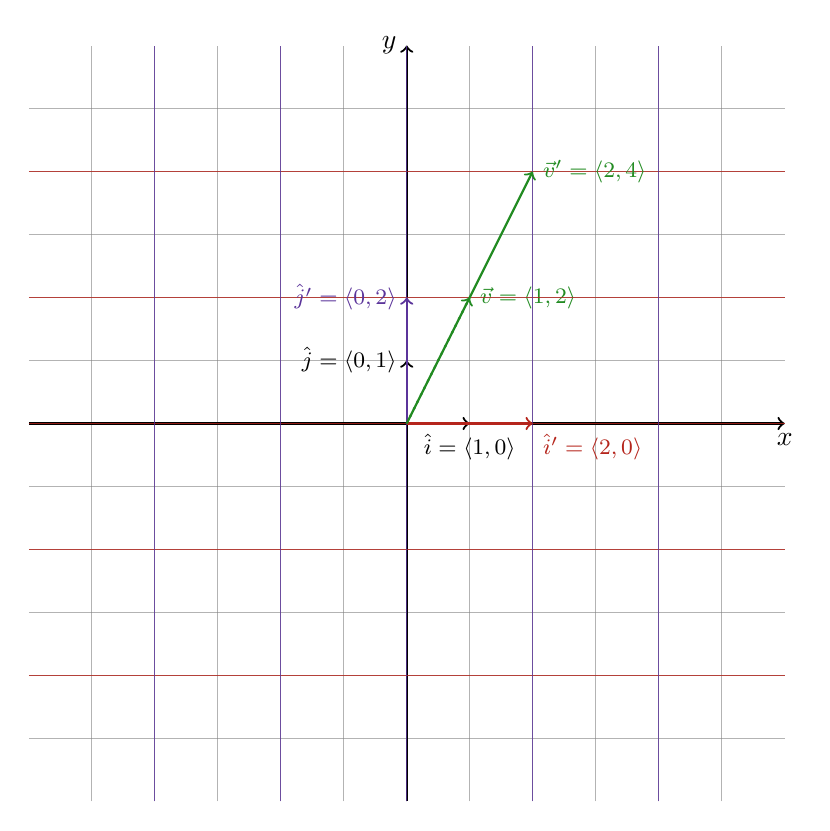
\begin{tikzpicture}[
        vector/.style={->, thick},
        scale=0.8
    ]

    \foreach \i in {-5, -4, ..., 5} {
        \draw[gray, thin, opacity=0.6] (\i, -6) -- (\i, 6);
        \draw[gray, thin, opacity=0.6] (-6, \i) -- (6, \i);
    }
    \draw[vector, black] (-6, 0) -- (6, 0) node[below] {$x$};
    \draw[vector, black] (0, -6) -- (0, 6) node[left] {$y$};

    \draw[vector] (0, 0) -- (1, 0) node[below]
        {\footnotesize $\hat{i} = \langle 1, 0 \rangle$};
    \draw[vector] (0, 0) -- (0, 1) node[left]
        {\footnotesize $\hat{j} = \langle 0, 1 \rangle$};
    \draw[vector, dotted, ForestGreen] (0, 0) -- (1, 2)
        node[right, ForestGreen]
            {\footnotesize $\vec{v} = \langle 1, 2 \rangle$};


    \foreach \j in {-4, -2, ..., 4} {
        \draw[BrickRed, opacity=0.8] (-6, \j) -- (6, \j);
    }
    \foreach \i in {-4, -2, ..., 4} {
        \draw[RoyalPurple, opacity=0.8] (\i, -6) -- (\i, 6);
    }

    \draw[vector, BrickRed] (0, 0) -- (2, 0)
        node[below right, BrickRed]
            {\footnotesize $\hat{i}' = \langle 2, 0 \rangle$};
    \draw[vector, RoyalPurple] (0, 0) -- (0, 2)
        node[left, RoyalPurple]
            {\footnotesize $\hat{j}' = \langle 0, 2 \rangle$};
    \draw[vector, ForestGreen] (0, 0) -- (2, 4)
        node[right, ForestGreen]
            {\footnotesize $\vec{v}' = \langle 2, 4 \rangle$};
\end{tikzpicture}
\end{figure}

There are other special linear transformations that output the same
vector space or the zero vector space.

\begin{definition}{}{}
A \textbf{zero transformation} is a linear transformation defined as
$Tv = \mathbf{0}$. An \textbf{identity transformation} is a linear
transformation that returns the same input vector as the output.
\end{definition}

Let's take a look at a few more examples on linear transformations.

\begin{problem}{}{}
Determine whether a transformation defined as $Tv = v^2$ is linear.
\end{problem}
\begin{solution}
Consider the following equation for arbitrary scalars $\alpha$ and
$\beta$.
\[
T(\alpha v_1 + \beta v_2)
= (\alpha v_1 + \beta v_2)^2
\]
Notice that the following equation holds.
\[
= \alpha T(v_1) + \beta T(v_2)
= \alpha v_1^2 + \beta v_2^2
\]
Because $(\alpha v_1 + \beta v_2)^2 \neq \alpha v_1^2 + \beta v_2^2$
in general, the transformation is not linear.
\end{solution}

Below is another example.

\begin{problem}{}{}
Determine whether a transformation defined as $Ty = \frac{dy}{dx}$
for some differentiable function $y = f(x)$ is linear.
\end{problem}
\begin{solution}
Consider the following equation for some scalars $\alpha$ and $\beta$.
\begin{align*}
    T(\alpha y_1 + \beta y_2)
    &= \frac{d}{dx} (\alpha y_1 + \beta y_2)
    = \frac{d}{dx} (\alpha y_1) + \frac{d}{dx} (\beta y_2) \\
    &= \alpha \frac{d}{dx} y_1 + \beta \frac{d}{dx} y_2
    = \alpha T(y_1) + \beta T(y_2)
\end{align*}
Thus, the transformation is linear.
\end{solution}

One thing that we can notice from the problem above is that the
transformation is not linear since changing the constants of an
input will not change the output. The transformation is also not
surjective as not all functions can be represented as the derivative
of other functions. Continuing, we can consider the following
transformation.

\begin{problem}{}{}
Determine whether a transformation defined as $T(\langle a, b \rangle)
= \langle -a, -b \rangle$ is linear.
\end{problem}
\begin{solution}
Consider the following equation for arbitrary scalars $\alpha$ and
$\beta$.
\begin{align*}
    T(\alpha \langle a, b \rangle + \beta \langle a', b' \rangle)
    &= T(\langle \alpha a, \alpha b \rangle +
        \langle \beta a', \beta b' \rangle)
    = T(\langle \alpha a + \beta a', \alpha b + \beta b' \rangle) \\
    &= \langle -\alpha a - \beta a', -\alpha b - \beta b' \rangle
    = \langle -\alpha a, -\alpha b \rangle +
        \langle -\beta a', - \beta b' \rangle \\
    &= \alpha \langle -a, -b \rangle + \beta \langle -a', -b' \rangle
    = \alpha T(v_1) + \beta T(v_2)
\end{align*}
Thus, the transformation is linear.
\end{solution}

Let's try and graph this to visually see how the vector space is
transformed.

\begin{figure}[H]
\centering
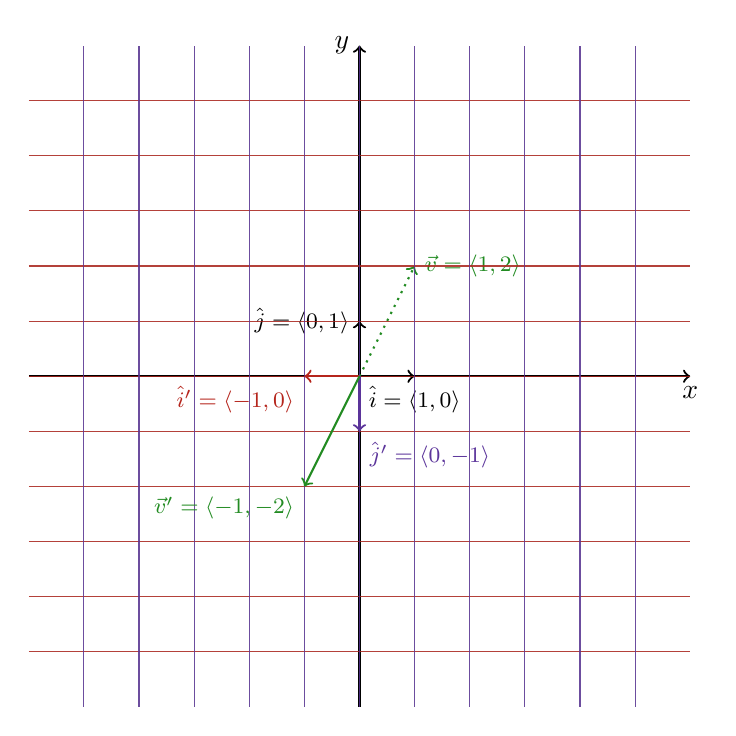
\begin{tikzpicture}[
        vector/.style={->, thick},
        scale=0.7
    ]

    \foreach \i in {-5, -4, ..., 5} {
        \draw[gray, thin, opacity=0.6] (\i, -6) -- (\i, 6);
        \draw[gray, thin, opacity=0.6] (-6, \i) -- (6, \i);
    }
    \draw[vector, black] (-6, 0) -- (6, 0) node[below] {$x$};
    \draw[vector, black] (0, -6) -- (0, 6) node[left] {$y$};

    \draw[vector] (0, 0) -- (1, 0) node[below]
        {\footnotesize $\hat{i} = \langle 1, 0 \rangle$};
    \draw[vector] (0, 0) -- (0, 1) node[left]
        {\footnotesize $\hat{j} = \langle 0, 1 \rangle$};
    \draw[vector, dotted, ForestGreen] (0, 0) -- (1, 2)
        node[right, ForestGreen]
            {\footnotesize $\vec{v} = \langle 1, 2 \rangle$};


    \foreach \j in {-5, -4, ..., 5} {
        \draw[BrickRed, opacity=0.8] (-6, \j) -- (6, \j);
    }
    \foreach \i in {-5, -4, ..., 5} {
        \draw[RoyalPurple, opacity=0.8] (\i, -6) -- (\i, 6);
    }

    \draw[vector, BrickRed] (0, 0) -- (-1, 0)
        node[below left, BrickRed]
            {\footnotesize $\hat{i}' = \langle -1, 0 \rangle$};
    \draw[vector, RoyalPurple] (0, 0) -- (0, -1)
        node[below right, RoyalPurple]
            {\footnotesize $\hat{j}' = \langle 0, -1 \rangle$};
    \draw[vector, ForestGreen] (0, 0) -- (-1, -2)
        node[below left, ForestGreen]
            {\footnotesize $\vec{v}' = \langle -1, -2 \rangle$};
\end{tikzpicture}
\end{figure}

This transformation reflects the vectors across the origin!
Now that we discussed what a linear transformation is, let's see how
matrices relate to it.

\subsection{Matrices and Linear Transformation}

Recall that every vector in a vector space can be represented as
a linear combination of the basis. We will apply our understanding
of a linear transformation to vector representations in a vector space
to find the relation.

Consider a basis $S = \{ v_1, \ldots, v_n \}$ for a vector space $V$.
Notice that by definition, an arbitrary vector $v \in V$ can be
represented as a linear combination of a basis as shown below
(where $c_k$ are constants).
\[
v = \sum_{k=1}^n c_k v_k
\]
Therefore, the following equation holds.
\[
(v)_S =
\begin{bmatrix}
    c_1 \\
    \vdots \\
    c_n
\end{bmatrix}
\]
Now returning to the definition of a linear transformation, we can
consider the following equation.
\[
Tv
= T \left( \sum_{k=1}^n c_k v_k \right)
= \sum_{k=1}^n c_k Tv_k
\]
Notice that the coordinate is preserved. In other words, the
following equation holds for the new basis $S' = \{ Tv_1, \ldots,
Tv_n \}$
\[
(Tv)_{S'} =
\begin{bmatrix}
    c_1 \\
    \vdots \\
    c_n
\end{bmatrix}
\]
This could let us geometrically understand that a linear transformation
``preserves'' the general shape of a vector space since the new
vectors have the same coordinates as the original ones, but with
different basis. With this in mind, we can establish two important
theorems.

\begin{theorem}{}{Coordinate Representation and Transformation}
For a vector space $V$ and a basis $S = \{ v_1, \ldots, v_n \}$,
the transformation $T: V \to \mathbb{R}^n$ defined as $Tv = (v)_S$
is linear and bijective.
\end{theorem}
\begin{proof}
First, the linearity of the transformation could be proven.
Consider the following equations for $u_1, u_2 \in V$ and some
constants $c_k$ and $d_k$.
\begin{align*}
    T(\alpha u_1 + \beta u_2)
    &= T \left(
        \alpha \sum_{k=1}^n c_k v_k + \beta \sum_{k=1}^n d_k v_k
    \right)
    = T \left( \sum_{k=1}^n (\alpha c_k + \beta d_k) v_k \right) \\
    &=
    \begin{bmatrix}
        \scriptstyle \alpha c_1 + \beta d_1 \\
        \scriptstyle \alpha c_2 + \beta d_2 \\
        \scriptstyle \vdots \\
        \scriptstyle \alpha c_n + \beta d_n
    \end{bmatrix}
    =
    \begin{bmatrix}
        \scriptstyle \alpha c_1 \\
        \scriptstyle \alpha c_2 \\
        \scriptstyle \vdots \\
        \scriptstyle \alpha c_n
    \end{bmatrix}
    +
    \begin{bmatrix}
        \scriptstyle \beta d_1 \\
        \scriptstyle \beta d_2 \\
        \scriptstyle \vdots \\
        \scriptstyle \beta d_n
    \end{bmatrix}
    =
    \alpha
    \begin{bmatrix}
        c_1 \\
        c_2 \\
        \vdots \\
        c_n
    \end{bmatrix}
    +
    \beta
    \begin{bmatrix}
        d_1 \\
        d_2 \\
        \vdots \\
        d_n
    \end{bmatrix} \\
    &= \alpha T(u_1) + \beta T(u_2)
\end{align*}
Thus, $T$ is linear. Continuing, notice that if $T(u_1) = T(u_2)$,
then $(u_1)_S = (u_2)_S$ and $u_1 = u_2$. Therefore, the
transformation is injective. The transformation is also surjective
as the entries $c_k$ in the coordinates are arbitrary real numbers.
Thus, $T$ is linear and bijective.
\end{proof}

Continuing, below is an important theorem and definition.

\begin{theorem}{}{Matrix Representation of $T$}
For vector spaces $V$ and $W$ with basis $B = \{ v_1, \ldots, v_n \}$
and $C = \{ w_1, \ldots, w_m \}$ respectively, there exists a matrix
$A$ such that the following equation holds for a linear transformation
$T: V \to W$ and arbitrary $v \in V$.
\vspace{-0.8\baselineskip}
\[
(Tv)_C = A(v)_B
\]
\end{theorem}
\begin{proof}
First and foremost, consider the following equation for any
$Tv_j \in W$ and constant $a_{ij}$.
\[
Tv_j = \sum_{i=1}^m a_{ij} w_i
\]
Let $A = [a_{ij}]$ and consider the following equation.
\[
A(v_2)_B
= A
\begin{bmatrix}
    0 \\
    1 \\
    \vdots \\
    0
\end{bmatrix}
=
\begin{bmatrix}
    a_{12} \\
    a_{22} \\
    \vdots \\
    a_{m2}
\end{bmatrix}
\]
Generalizing, $(Tv_j)_C = A(v_j)_B$ and the following equations hold
for constants $c_j$.
\begin{align*}
    (Tv)_C
    &= \left( \sum_{j=1}^n c_j Tv_j \right)_C
    = \sum_{j=1}^n (c_j Tv_j)_C
    = \sum_{j=1}^n c_j (Tv_j)_C \\
    &= \sum_{j=1}^n c_j A(v_j)_B
    = A \left( \sum_{j=1}^n (c_j v_j)_B \right)
    = A \left( \sum_{j=1}^n c_j v_j \right)_B \\
    &= A(v)_B
\end{align*}
Thus, there always exists such a matrix $A$.
\end{proof}

The matrix $A$ above has a special name. The matrix is known as
the matrix representation of $T$ with respect to $B$ and $C$,
denoted as $A_B^C$. In short, we also say $A$ from $B$ to $C$.

Continuing from the theorem, we can also notice that for a vector
space $V$ and its basis $A$ and $B$, there exists a matrix $P_A^B$
such that $(v)_B = P_A^B (v)_A$ holds for all $v \in V$.
To prove this, consider the identity transformation $T: V \to V$.
By theorem \ref{theo:Matrix Representation of $T$}, there exists a
matrix $P$ such that $(v)_B = P_A^B (v)_A$. This matrix too has a
special name.

\begin{definition}{}{}
A \textbf{transition matrix} is a matrix that converts the coordinate
representation of a vector in a vector space $V$ from a basis in $V$
to another basis in $V$.
\end{definition}

Now from the definitions, we could notice that linear transformations
are highly related to the basis of a vector space. If we know how
the basis is mapped, we can understand the linear transformation.
Consider the following theorem.

\begin{theorem}{}{Transition Matrix and Basis I}
For a vector space and its bases $A$ and $B$, the coordinate
representation of the $j$ vector of $A$ with respect to $B$ is the
$j^\text{th}$ column of the transition matrix $P_A^B$.
\end{theorem}
\begin{proof}
Let $A = \{ a_1, \ldots, a_n \}$ and $B = \{ b_1, \ldots, b_n \}$.
For some scalars $p_{ij}$, $a_i$ can be written as $a_j = \sum_{i=1}^n
p_{ij} b_i$. Let a vector $v$ in the vector space be written as $v =
\sum_{k=1}^n a'_k + a_k = \sum_{k=1}^n b'_k + b_k$. Continuing, the
following equation holds.
\[
v
= \sum_{j=1}^n a'_j a_j
= \sum_{j=1}^n a'_j \left( \sum_{i=1}^n p_{ij} b_i \right)
= \sum_{i=1}^n \left( \sum_{j=1}^n p_{ij} a'_j \right) b_i
\]
In other words, $b'_i = \sum_{j=1}^n p_{ij} a'_j$ and $(v)_B =
[p_{ij}] (v)_A = P_A^B (v)_A$.
\end{proof}

Continuing with the theorem above, we can derive the following.

\begin{theorem}{}{Inverse of Transition Matrix}
A transition matrix $P_A^B$ is always invertible and $(P_A^B)^{-1}
= P_B^A$.
\end{theorem}
\begin{proof}
Consider the following equations for a vector $v$.
\begin{align*}
    (v)_B &= P_A^B (v)_A \\
    (v)_A &= P_B^A (v)_B
\end{align*}
Therefore, $(v)_B = P_A^B (v)_A = P_A^B P_B^A (v)_B$ for all $(v)_B$.
Thus, $P_A^B P_B^A = I$ and the theorem holds.
\end{proof}

Now how about matrix representations like $A_S^S$? We have an
interesting theorem that links such matrices with transition matrices.

\begin{theorem}{}{Transition Matrix and Basis II}
Let $A_B^B$ and $A_C^C$ be the matrix representations of linear
transformations for bases $B$ and $C$. If $P_B^C$ represents the
transition matrix, then $A_B^B = P_C^B A_C^C P_B^C$.
\end{theorem}
\begin{proof}
For a vector $v$ in the same vector space, notice that $(Tv)_B =
A_B^B (v)_B$ and $(v)_C = P_B^C (v)_B$ hold by definition.
Consider the following equation.
\[
(Tv)_B
= P_C^B (Tv)_C = P_C^B A_C^C (v)_C
= P_C^B A_C^C P_B^C (v)_B
= A_B^B (v)_B
\]
Thus, $P_C^B A_C^C P_B^C = A_B^B$.
\end{proof}

Let's use $A$ for $A_B^B$, $\tilde{A}$ for $A_C^C$, and $P$ for
$P_B^C$ where $P^{-1} = P_C^B$. Notice that we can write $A = P^{-1}
\tilde{A} P$ and $PA = \tilde{A} P$. Here, we say that $A$ and
$\tilde{A}$ are \textbf{similar}.

\begin{definition}{}{}
Two matrices $A$ and $B$ are \textbf{similar} if the linear
transformation that they represent with different bases is identical.
In other words, for transition matrix $P = P_A^B$, $PA = BP$.
\end{definition}

Continuing with the definition, we can establish the following
theorem.

\begin{theorem}{}{Similar Matrices and Linear Transformation}
For a vector space $V$ with basis $B$, let $A$ be the matrix
representation of the linear transformation $T: V \to V$ from $B$ to
$B$. If $A$ is similar to another matrix representation $\tilde{A}$,
then there exists a basis $C$ such that $\tilde{A}$ represents the
same linear transformation from $C$ to $C$.
\end{theorem}
\begin{proof}
First and foremost, let a transition matrix from a basis $C$ to $B$
be $P$ and let $v$ be a vector in the vector space. Consider the
following equations.
\begin{align*}
    (Tv)_B
    &= A (v)_B = AP (v)_C \\
    &= P (Tv)_C
\end{align*}
Therefore, $AP (v)_C = P (Tv)_C$ and $(Tv)_C = A' (v)_C =
P^{-1} A P (v)_C$. In other words, for each basis $C$, there exists
a transition matrix similar to $A$. Moreover, because the whole
process is invertible, the theorem holds.
\end{proof}

Now that we discussed that matrices can be used to represent linear
transformations, let's discuss about topics that are never left out
in linear algebra.

\subsection{Kernels and Images}

As you could have noticed, sometimes it is easier to discuss a linear
transformation with intuitions and sometimes matrices are much more
straightforward. Recall that linear transformations are functions
for vector spaces. Sometimes it is easier to look at the functions
directly and sometimes it is more convenient to look at the matrix
representation of such functions. That is what we are going to do
with kernels and images. As always, let's get started with
definitions.

\begin{definition}{}{}
The \textbf{kernel} of a linear transformation $T: V \to W$, also
known as the \textbf{nullspace} of $T$, is the set of vectors in
$V$ that are mapped to zero vectors when transformed with $T$.
\vspace{-0.8\baselineskip}
\[
\ker(T)
= \{ v \in V \mid Tv = \mathbf{0} \}
\]
\end{definition}

Continuing with the definition, we can establish two fundamental
properties of the kernel of a transformation.

\begin{theorem}{}{Properties of the Kernel}
Consider the following statements for all linear transformations
$T: V \to W$.
\begin{enumerate}[noitemsep]
\item $\mathbf{0} \in \ker(T)$
\item $\ker(T)$ is a subspace of $V$.
\end{enumerate}
\end{theorem}

Let's start by proving the first statement. The proof is rather
straightforward with the properties of linear transformation.

\begin{proof}
Consider the following equation.
\[
T(\mathbf{0})
= T(0 \mathbf{0})
= 0 T(\mathbf{0})
= \mathbf{0}
\]
Because $\mathbf{0}$ is mapped to $\mathbf{0}$ after any linear
transformation $T$, $\mathbf{0} \in \ker(T)$ for all linear
transformations $T$.
\end{proof}

Continuing, below is the proof for the second statement.

\begin{proof}
By definition, $\ker(T) \in V$. Therefore, it suffices to show that
the kernel of $T$ is closed under vector addition and scalar
multiplication. Because $\ker(T)$ is not empty by the first statement,
consider the following equations for $u, v \in \ker(T)$ and some
scalars $\alpha$ and $\beta$.
\[
T(\alpha u + \beta v)
= \alpha Tu + \beta Tv
= \alpha \mathbf{0} + \beta \mathbf{0}
= \mathbf{0}
\]
In other words $\alpha u + \beta v \in \ker(T)$ and $\ker(T)$ is a
subspace of $V$.
\end{proof}

Recall that a linear transformation can be represented as some
matrix $A$. Therefore, kernel of $A$ can be interpreted as the
set of solutions to $Ax = \mathbf{0}$. Notice that some solutions
retain finite and infinite number of vectors. Therefore, we can
establish the following definition.

\begin{definition}{}{}
The \textbf{nullity} of $T$, denoted as $\Null(T)$, is the dimension
of $\ker(T)$ for some linear transformation $T$.
\end{definition}

Continuing, we can define the image of a transformation, which should
be unsurprising.

\begin{definition}{}{}
The subset of the codomain $W$ for a transformation $T: V \to W$ that
contains all output vectors is known as the \textbf{image} of $T$.
Below defines $\Im(T)$ with $v \in V$.
\vspace{-0.8\baselineskip}
\[
\Im(T)
= \{ w \in W \mid w = Tv \}
\]
\end{definition}

Although the kernel and the image of a transformation are very
different, we can establish very similar statements for the image
just as how we derived them for the kernel.

\begin{theorem}{}{Properties of the Image}
Consider the following statements for all linear transformations
$T: V \to W$.
\begin{enumerate}[noitemsep]
\item $\mathbf{0} \in \Im(T)$
\item $\Im(T)$ is a subspace of $W$.
\end{enumerate}
\end{theorem}

Let's start by proving the first statement.

\begin{proof}
By theorem \ref{theo:Properties of the Kernel}, there exists a
vector in $V$ such that it is mapped to $\mathbf{0}$ in $W$. Thus,
the statement holds.
\end{proof}

Continuing, below is the proof for the second statement.

\begin{proof}
First and foremost, $\Im(T) \in W$ by definition. Therefore,
it suffices to show that the image is closed under vector addition
and scalar multiplication. Consider the following equation for
$v_1, v_2 \in V$, $Tv_1 = w_1$, $Tv_2 = w_2$, and some scalars
$\alpha$ and $\beta$.
\[
\alpha w_1 + \beta w_2
= \alpha Tv_1 + \beta Tv_2
= T(\alpha v_1 + \beta v_2)
\]
Because $T(\alpha v_1 + \beta v_2) \in \Im(T)$, $\alpha w_1 +
\beta w_2 \in \Im(T)$ and the statement holds.
\end{proof}

Now recall the kernel of a matrix $A$ is the set of all solutions to
the equation $Ax = \mathbf{0}$. Similarly, the image is the set of
all possible outcomes of the product $Ax$ for some $x \in V$.
Consider the equations below.
\[
\begin{bmatrix}
    a_{11} & a_{12} & \cdots & a_{1n} \\
    a_{21} & a_{22} & \cdots & a_{2n} \\
    \vdots & \vdots & \ddots & \vdots \\
    a_{m1} & a_{m2} & \cdots & a_{mn}
\end{bmatrix}
\begin{bmatrix}
    x_1 \\
    x_2 \\
    \vdots \\
    x_n
\end{bmatrix}
=
\begin{bmatrix}
    \sum_{k=1}^n a_{1k} x_k \\
    \sum_{k=1}^n a_{2k} x_k \\
    \vdots \\
    \sum_{k=1}^n a_{mk} x_k
\end{bmatrix}
=
\sum_{k=1}^n
x_k
\begin{bmatrix}
    a_{1k} \\
    a_{2k} \\
    \vdots \\
    a_{mk}
\end{bmatrix}
\]
In other words, the image of $A$ is the column space of $A$.
Therefore, we can establish the following definition.

\begin{definition}{}{}
The \textbf{rank} of a transformation $T$, denoted as $\Rank(T)$,
is $\dim(\Im(T))$.
\end{definition}

Continuing from the definition and ideas of column space and the
image, we can derive the following theorem.

\begin{theorem}{}{Rank and Matrix Representation}
Let $B$ and $C$ be $n$-dimensional and $m$-dimensional bases for
$V$ and $W$ in a linear transformation $T: V \to W$ respectively.
If the matrix representation of $T$ is $A = A_B^C$, then
$\Rank(T) = \Rank(A)$.
\end{theorem}
\begin{proof}
First and foremost, let a basis for $\Im(T)$ be $\{ w_1, \ldots,
w_k \}$. Notice that if $\{ (w_1)_C, \ldots, (w_k)_C \}$ is a
basis for $\Col(A)$, then $\dim(\Im(T)) = \dim(\Col(A))$ and
$\Rank(T) = \Rank(A)$. Thus, it suffices to show that $\{ (w_1)_C,
\ldots, (w_k)_C \}$ is a basis for $\Col(A)$.

Let $c_k$ be some scalars that $x \in \Col(A)$ is represented
as the linear combination of the columns $A_k$ of $A$ where
$x = \sum_{k=1}^n c_k A_k$. Note that $c_k$ can be written as
an $n$-tuple. Thus, let $v \in V$ be a vector such that the
following equation holds.
\[
(v)_B =
\begin{bmatrix}
    c_1 \\
    c_2 \\
    \vdots \\
    c_n
\end{bmatrix}
\]
Continuing, $x = A(v)_B = (Tv)_C$. Because $Tv \in \Im(T)$,
it is evident that $x$ lies in $\Span\{ (w_1)_C, \ldots, (w_k)_C \}$.
Moreover, because $x$ is an arbitrary vector from $\Col(A)$, it is
evident that $\Col(A) \subset \Span\{ (w_1)_C, \ldots, (w_k)_C \}$ and
$\{ (w_1)_C, \ldots, (w_k)_C \}$ spans $\Col(A)$.

By definition, $\{ w_1, \ldots, w_k \}$ is linearly independent.
For some scalars $d_k$, for $\sum_{k=1}^n d_k (w_k)_C$ to be
a zero vector, $(\sum_{k=1}^n d_k w_k)_C = \mathbf{0}$ and
$\sum_{k=1}^n d_k w_k = \mathbf{0}$, which only happens when
$d_k = 0$ for all integer $k \in [0, n]$. Thus, $\{ (w_1)_C,
\ldots, (w_k)_C \}$ is linearly independent and is a basis for
$\Col(A)$.
\end{proof}

As you can see above by the theorem, although the kernel and the
image of a linear transformation appear to be totally unrelated,
they are somehow related. Below is another theorem that connects
the bases of the kernel and the image of a linear transformation.

\begin{theorem}{}{Basis of the Kernel and the Image}
Let $\{ v_1, \ldots, v_k \}$ be the basis of the kernel of a
linear transformation $T: V \to W$. If $\{ v_1, \ldots, v_k, \ldots
v_n \}$ is a basis for $V$, then a basis of $\Im(T)$ is $\{ Tv_{k+1},
\ldots, Tv_n \}$.
\end{theorem}
\begin{proof}
To prove that $\{ Tv_{k+1}, \ldots, Tv_n \}$ is a basis of $\Im(T)$,
it suffices to show that the set of vectors is linearly independent
and spans $\Im(T)$. First, to show that the set is linearly
independent, consider the following equations for some scalars $c_i$.
\[
\sum_{i=k+1}^n c_i Tv_i
= T \left( \sum_{i=k+1}^n c_i v_i \right)
= \mathbf{0}
\]
In other words, $\sum_{i=k+1}^n c_i v_i \in \ker(T)$ and it can
be written as the linear combination of the basis, or $\sum_{i=k+1}^n
c_i v_i = \sum_{i=1}^k c_i v_i$. By definition, because $\{ v_1,
\ldots, v_k, \ldots v_n \}$ is linearly independent, $c_i$ must be
all zero for integer $i \in [1, n]$ for $\sum_{i=k+1}^n c_i v_i -
\sum_{i=1}^k c_i v_i = \mathbf{0}$ to satisfy. Thus, $\{ Tv_{k+1},
\ldots, Tv_n \}$ is linearly independent.

Continuing, the fact that the set $\{ Tv_{k+1}, \ldots, Tv_n \}$
spans $\Im(T)$ can be proven. Let $w = Tv$ for any $w \in \Im(T)$.
Consider the following equations below.
\begin{align*}
    w
    &= Tv
    = T \left( \sum_{i=1}^n c_i v_i \right)
    = \sum_{i=1}^n c_i Tv_i \\
    &= \sum_{i=1}^k c_i Tv_i + \sum_{i=k+1}^n c_i Tv_i
    = \sum_{i=k+1}^n c_i Tv_i
    \in \Span\{ Tv_{k+1}, \ldots, Tv_n \}
\end{align*}
In other words, $\{ Tv_{k+1}, \ldots, Tv_n \}$ spans $\Im(T)$. Thus,
the theorem holds.
\end{proof}

Continuing from this theorem, we can establish another interesting
corollary as a theorem.

\begin{theorem}{}{Rank and Nullity of T}
For a finite dimensional vector space $V$, the following equation
is true for a linear transformation $T: V \to W$.
\vspace{-0.8\baselineskip}
\[
\Rank(T) + \Null(T) = \dim(V)
\]
\end{theorem}
\begin{proof}
Let $k = \dim(\ker(T))$ and $n = \dim(V)$. By Theorem \ref{theo:Basis
of the Kernel and the Image}, there exists a basis for $\Im(T)$ with
$n - k$ vectors, or $\Rank(T) = \dim(\Im(T)) = n - k$. Thus,
$\Rank(T) + \Null(T) = n - k + k = n = \dim(V)$.
\end{proof}

Moving on from the relationship with the kernel and the image of a
linear transformation, let's discuss about injection, surjection,
and bijection. Consider the following theorem.

\begin{theorem}{}{Linear Transformation and Injection}
A linear transformation $T: V \to W$ is injective if and only if
$\ker(T) = \{ \mathbf{0} \}$.
\end{theorem}
\begin{proof}
By definition, $T$ is injective if $v_1, v_2 \in V$ such that
$v_1 \neq v_2$ implies $Tv_1 \neq Tv_2$. Therefore, if $v \in
\ker(T)$, then $Tv = \mathbf{0} = T\mathbf{0}$ and $\ker(T)$
must contain no nonzero vectors for $T$ to be injective.
Thus, $\ker(T)$ must only contain the zero vector.
\end{proof}

Continuing, below is another theorem on injection and surjection.

\begin{theorem}{}{Injection and Surjection of a Linear Transformation}
For a linear transformation $T: V \to W$ with $\dim(V) = \dim(W) = n$,
$T$ is injective if and only if $T$ is surjective.
\end{theorem}
\begin{proof}
By Theorem \ref{theo:Linear Transformation and Injection}, $T$ is
injective if and only if $\ker(T) = \{ \mathbf{0} \}$. Moreover by
definition, $\ker(T) = \{ \mathbf{0} \}$ if and only if $\Null(T) = 0$
and $\Rank(T) = \dim(V) - \Null(T) = n$ by Theorem \ref{theo:Rank and
Nullity of T}. Continuing by definition, $\Rank(T) = n$ if and only if
$\dim(\Im(T)) = n = \dim(W)$. Therefore, $T$ is injective if and only
if $T$ is surjective.
\end{proof}

With the interesting properties, we can assign a special name for
bijective linear transformation.

\begin{definition}{}{}
A bijective linear transformation is called an \textbf{isomorphism}.
Moreover, a vector space $V$ is said to be \textbf{isomorphic} to
another vector space $W$ if there exists an isomorphism $T: V \to W$,
denoted as $V \cong W$.
\end{definition}

Continuing from the definition, we can derive the following
properties.

\begin{theorem}{}{Reflex, Symmetry, and Transition of Isomorphism}
For vector spaces $U$, $V$, and $W$, isomorphism is reflexive,
symmetric, and transitive.
\begin{enumerate}[noitemsep]
\item $U \cong U$
\item If $U \cong V$, then $V \cong U$.
\item If $U \cong V$ and $V \cong W$, then $U \cong W$.
\end{enumerate}
\end{theorem}

Let's start by proving the first statement.

\begin{proof}
Notice that it suffices to show that the identity transformation
is bijective. By definition, because each vector is mapped to
itself, identity transformation is bijective and $U \cong U$.
\end{proof}

Below is the proof for the second property.

\begin{proof}
First and foremost, notice that if there exists $T: U \to V$ that
is bijective, then there exists its inverse $T^{-1}: V \to U$
that is also bijective. Continuing, consider the equation below
for some vectors $v_1, v_2 \in V$ and scalars $\alpha$ and $\beta$.
\begin{align*}
    \alpha T^{-1} v_1 + \beta T^{-1} v_2
    &= T^{-1} \left(
        T \left( \alpha T^{-1} v_1 + \beta T^{-1} v_2 \right)
    \right) \\
    &= T^{-1} \left(
        \alpha T \left( T^{-1} v_1 \right) +
            \beta T \left( T^{-1} v_2 \right)
    \right) \\
    &= T^{-1} \left( \alpha v_1 + \beta v_2 \right)
\end{align*}
Therefore, $T^{-1}$ is linear and $T^{-1}$ is an isomorphism.
\end{proof}

Continuing, below is the proof for the last statement.

\begin{proof}
First and foremost, let $T_1: U \to V$ and $T_2: V \to W$ be
isomorphisms. Therefore, it suffices to show that $T_2 \circ T_1$
is an isomorphism. Notice that because $T_1$ and $T_2$ are
bijective, $T_2 \circ T_1$ must also be bijective. Moreover,
consider the following equation for some vectors $v_1, v_2 \in V$
and scalars $\alpha$ and $\beta$.
\begin{align*}
    (T_2 \circ T_1) (\alpha v_1 + \beta v_2)
    &= T_2 (\alpha T_1v_1 + \beta T_1v_2) \\
    &= \alpha T_2 (T_1v_1) + \beta T_2 (T_1v_2) \\
    &= \alpha (T_2 \circ T_1) (v_1) + \beta (T_2 \circ T_1) (v_2)
\end{align*}
Thus, $T_2 \circ T_1$ is linear and the statement is true.
\end{proof}

As you can see above, the three statements in Theorem
\ref{theo:Reflex, Symmetry, and Transition of Isomorphism} each
shows a relation called reflexive, symmetric, and transitive.
Continuing from this terms, we can assign a special name for a
relation.

\begin{definition}{}{}
An \textbf{equivalence relation} is a relation that is reflexive,
symmetric, and transitive.
\end{definition}

Below is another interesting theorem on isomorphism.

\begin{theorem}{}{Dimension and Isomorphism}
For finite dimensional vector spaces $V$ and $W$, $V \cong W$ if and
only if $\dim(V) = \dim(W)$.
\end{theorem}
\begin{proof}
First, the statement if $\dim(V) = \dim(W)$, then $V \cong W$ can be
proven. Notice that the coordinate representations of infinitely many
vectors in $V$ and $W$ are unique. Therefore, $V \cong \mathbb{R}^n$
and $W \cong \mathbb{R}^n$. By Theorem \ref{theo:Reflex, Symmetry, and
Transition of Isomorphism}, $\mathbb{R}^n \cong W$ and $V \cong W$.

Continuing, if $V \cong W$, then there exists a linear transformation
$T: V \to W$ that is bijective. By Theorem \ref{theo:Linear
Transformation and Injection}, $\ker(T) = \{ \mathbf{0} \}$ and
$\Null(T) = 0$. Moreover by definition, because $T$ is surjective,
$\Rank(T) = \dim(\Im(T)) = \dim(W)$. Finally by Theorem \ref{theo:Rank
and Nullity of T}, $\dim(W) + 0 = \dim(V)$ and the theorem holds.
\end{proof}

From the theorem above, we can notice that if we consider a bijective
linear transformation that maps to coordinate representation, then
all $n$-dimensional vector spaces are isomorphic to $\mathbb{R}^n$.
In other words, every $n$-dimensional vector space over a given
field for some finite $n$ can be considered as the same vector space,
but just with different representations.

This is it for linear transformations, and let's discuss about
eigenvalues and eigenvectors!

\end{document}


